\RequirePackage{plautopatch}
% \documentclass[report,paper=a4, fontsize=12pt, line_length=16cm, number_of_lines=33]{jlreq}
% \usepackage[haranoaji,deluxe]{luatexja-preset}
% \usepackage{amsmath,amssymb}
% \usepackage{libertinus}

\documentclass[report,paper=a4, fontsize=12pt, line_length=16cm, number_of_lines=33,dvipdfmx]{jlreq}
\usepackage{jlreq-deluxe}
\usepackage{amsmath,amssymb}
\usepackage{stix2}
\renewcommand{\bfdefault}{bx}
% \usepackage{libertine}
% \usepackage{libertinust1math}
% \usepackage[T1]{fontenc}
% \usepackage{mlmodern}
% \usepackage[T1]{fontenc}
% \usepackage{tgtermes,tgheros,tgcursor}
% \renewcommand{\bfdefault}{bx}
% \usepackage[libertine]{newtxmath}

%% Fonts
%\usepackage{lmodern}
%\usepackage[T1]{fontenc}

\usepackage{tikz}

\usepackage{graphicx}
\graphicspath{{fig/}}

\usepackage{physics}
\usepackage{color}

\usepackage{tcolorbox}
\tcbuselibrary{breakable, skins, theorems}
%\usepackage{cleveref}

% font warningを出さないため
% \DeclareFontShape{JY2}{hgt}{b}{n}{<->ssub*hgt/bx/n}{}
% \DeclareFontShape{JY2}{hgt}{m}{it}{<->ssub*hgt/m/n}{}
% \DeclareFontShape{JT2}{hgt}{b}{n}{<->ssub*hgt/bx/n}{}
% \DeclareFontShape{JT2}{hgt}{m}{it}{<->ssub*hgt/m/n}{}
\newcommand{\qed}{■}
\newcommand{\kyou}[1]{{\sffamily \bfseries #1}}

\numberwithin{equation}{chapter}
%%%%%%%%%%%%%%%%%%%%%%%%%%%%%%%%%%%%%%%%%%%%%%%%%%%%%%%%%%%%%%%%%%%%%%
%                          often used macro
\newcommand{\del}{\partial}
\newcommand{\Cb}{\mathbb{C}}
\newcommand{\Zb}{\mathbb{Z}}
\newcommand{\CP}{\Cb \mathrm{P}}
%\newcommand{\strong}[1]{{\sffamily \gtfamily \bfseries #1}}
\newcommand{\Ztwo}{\mbox{$\mathbb{Z}_{2}$}}
\newcommand{\Hh}{\widehat{H}}
\newcommand{\Uh}{\widehat{U}}
\newcommand{\Vh}{\widehat{V}}
\newcommand{\Jh}{\widehat{J}}
\newcommand{\Qh}{\widehat{Q}}
\newcommand{\Oh}{\widehat{\mathcal{O}}}
\newcommand{\Gh}{\widehat{G}}
\newcommand{\ah}{\hat{a}}
\newcommand{\bh}{\hat{b}}
\newcommand{\Ocal}{\mathcal{O}}
\newcommand{\Ocalh}{\widehat{\mathcal{O}}}
\newcommand{\U}{\mbox{U}}
\newcommand{\ZIsing}{Z_{\mathrm{Ising}}}
\newcommand{\Zgauged}{Z_{\mathrm{Ising}/\Zb_2}}
\newcommand{\deltamod}[1]{\delta^{\mathrm{mod} \ 2}_{#1}}
\newcommand{\Kt}{\widetilde{K}}
\newcommand{\link}[1]{\expval{#1}}
\newcommand{\plaq}[1]{\expval{#1}}

\newcommand{\Ising}{\mbox{Ising}}
\newcommand{\gIsing}{\mbox{Ising$/\Zb_2$}}

\newcommand{\Tcal}{\mathcal{T}}


\begin{document}

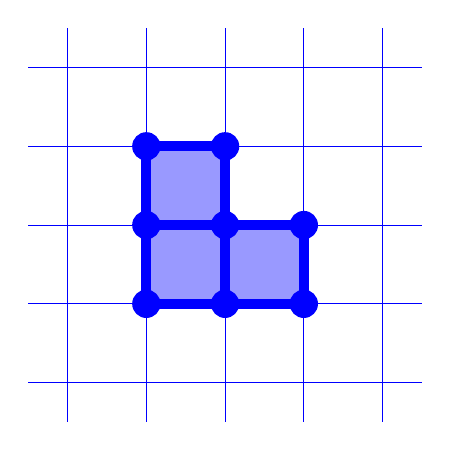
\begin{tikzpicture}
    \draw[step=1, blue] (-1.5,-1.5) grid (3.5,3.5); 
    \foreach \x/\y in {0/0, 0/1, 1/0}{
        \fill[blue!40](\x,\y) rectangle (\x+1,\y+1);
    }
    \foreach \x/\y in {0/0, 0/1, 1/0, 1/1, 0/2, 1/2, 2/0, 2/1}{
        \fill[blue] (\x,\y) circle (1.8mm);
    }
    \foreach \x/\y in {0/0, 0/1, 0/2, 1/0, 1/1}{
    \draw[blue, line width = 1.3mm](\x,\y)--(\x + 1,\y);
    }
    \foreach \x/\y in {0/0, 0/1, 1/0, 1/1, 2/0}{
    \draw[blue, line width = 1.3mm](\x,\y)--(\x,\y+1);
    }
\end{tikzpicture}

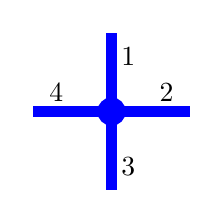
\begin{tikzpicture}
    \fill[blue] (0,0) circle (1.8mm);
    \foreach \x/\y in {1/0, 0/1, -1/0, 0/-1}{
    \draw[blue, line width = 1.3mm](0,0)--(\x,\y);
    }
    \node (A) at (0,0.7)[right]{$1$};
    \node (B) at (0,-0.7)[right]{$3$};
    \node (C) at (0.7,0)[above]{$2$};
    \node (D) at (-0.7,0)[above]{$4$};
\end{tikzpicture}

\end{document}  